% CAPÍTULO 2 — FUNDAMENTAÇÃO TEÓRICO -----------------------------------------------------------------------

\chapter{Fundamentação Teórica}
\label{cap:referencial}

\section{Mercado de trabalho em TI: crescimento e desigualdade}

Nas últimas décadas, o setor de TI no Brasil cresceu sem grandes interrupções, puxado pela transformação digital de empresas e órgãos públicos, pelo comércio eletrônico e pelos modelos de negócio centrados em plataformas digitais. Segundo o Relatório Setorial 2024 da BRASSCOM, o macrossetor de Tecnologia da Informação e Comunicação (TIC) responde por 6,5\% do Produto Interno Bruto (PIB) brasileiro e reunia, em 2024, cerca de 2,1 milhões de empregos formais \cite{Brasscom2024}.

Uma pesquisa da Federação do Comércio de Bens, Serviços e Turismo do Estado de São Paulo (FECOMERCIOSP), baseada nos microdados da RAIS, mostrou que as profissões ligadas à tecnologia cresceram 95\% entre 2012 e 2022, com altas acima de 740\% em casos como o de engenheiro de sistemas operacionais \cite{Fecomercio2024}. A oferta de mão de obra qualificada não acompanhou esse ritmo: entre 2019 e 2024, o mercado precisou de cerca de 665 mil profissionais de TI, mas formaram-se 465 mil entre 2018 e 2023 (quem se forma em um ano entra no mercado no seguinte), um déficit de cerca de 30\% \cite{Brasscom2025}.

A pandemia de COVID-19 acelerou esse cenário. A partir de 2020, a adoção de ferramentas de colaboração remota, \textit{cloud computing} e automação ampliou a procura por profissionais de TI no momento em que o restante do mercado formal se contraía \cite{CAGED2024}.

\label{sec:literatura-trabalho}
Além do crescimento, três temas da economia do trabalho orientam a leitura dos resultados: como se formam os hiatos salariais por sexo e por raça, o que acontece com o emprego e o salário quando uma função passa a ser contratada de fora, e o que o trabalho remoto muda na geografia do emprego.

Sobre o hiato de gênero, a revisão de \citeonline{BlauKahn2017} mostra que, nos Estados Unidos, ele caiu de forma expressiva entre 1980 e 2010, em boa parte porque as mulheres alcançaram e ultrapassaram os homens em escolaridade e experiência. Com isso, o capital humano passou a explicar pouco da diferença restante, e a parcela não explicada ganhou peso relativo. \citeonline{Goldin2014} localiza essa parcela dentro das ocupações, na forma como cada uma remunera jornadas longas e pouco flexíveis, e, para o Brasil, \citeonline{Madalozzo2010} mostra que a parcela não explicada, mesmo com controle de ocupação, caiu de 33\% em 1978 para pouco mais de 16\% em 2007 e ficou estável na última década do período. Esses trabalhos mostram por que um hiato pode crescer sem que nenhuma regra de remuneração mude: basta que a vantagem de características de um grupo encolha.

Sobre raça, a desigualdade de rendimentos no Brasil é de outra magnitude. Em 2021, o rendimento médio de trabalhadores brancos superava em 75,7\% o de pretos e em 70,8\% o de pardos, e a diferença persistia entre pessoas com ensino superior completo \cite{IBGE2022Desigualdades}. Uma parte dela vem de onde cada grupo trabalha, e outra de quanto recebe na mesma posição, separação que a decomposição de Oaxaca-Blinder (\autoref{subsec:oaxaca}) permite medir.

Sobre a terceirização, \citeonline{AbrahamTaylor1996} mostram que as empresas contratam serviços de fora por três motivos: reduzir custos salariais, ajustar a força de trabalho às oscilações de demanda e ter acesso a competências especializadas que não compensaria manter internamente. Os dois últimos descrevem bem os serviços de tecnologia. Em ocupações de serviços, quem passa a trabalhar para o fornecedor ganha menos: na Alemanha, trabalhadores terceirizados de limpeza, segurança, alimentação e logística passaram a receber de 10\% a 15\% menos que os não terceirizados em postos equivalentes \cite{GoldschmidtSchmieder2017}, e resultado na mesma direção foi encontrado para faxineiros e vigilantes nos Estados Unidos \cite{DubeKaplan2010}. Se o mesmo vale para ocupações qualificadas, como as de TI, é uma questão em aberto.

Uma ressalva de método acompanha qualquer série de salários: a composição da força de trabalho muda com o ciclo. Na expansão, entram mais trabalhadores de salário baixo e pouco tempo de casa; na recessão, são eles os primeiros a sair. Por isso médias e medianas agregadas podem ficar estáveis enquanto os salários de cada grupo se movem, ou o contrário \cite{Solon1994}. O mesmo vale para o tempo médio de emprego.

Por fim, o trabalho remoto que se expandiu com a pandemia não voltou ao nível anterior: nos Estados Unidos, estabilizou-se em uma fração dos dias trabalhados muitas vezes maior que antes de 2020, concentrada em ocupações de alta qualificação \cite{Barrero2023}. Para quem estuda o emprego por registros administrativos, a consequência é direta: o lugar do empregador e o lugar onde a pessoa vive e trabalha deixam de coincidir.

Estudar essas dinâmicas exige fontes com cobertura nacional, série histórica longa e detalhe por ocupação, e RAIS e CAGED são as únicas bases brasileiras que atendem aos três requisitos ao mesmo tempo \cite{SilvaLima2018}.

\section{Bases de dados governamentais: RAIS e CAGED}

A RAIS é um registro administrativo criado pelo Decreto n.º 76.900/1975, de preenchimento anual e obrigatório para todos os estabelecimentos com empregados formais, sejam celetistas, estatutários, avulsos ou outros. A cada ano-base, são declarados os vínculos ativos em 31 de dezembro e os encerrados ao longo do ano, com cargo (CBO), salário de dezembro, carga horária, grau de instrução, gênero, raça/cor, tempo de emprego, município e CNAE do estabelecimento \cite{RAIS2024}. A série existe desde 1985, com boa qualidade a partir dos anos 2000, o que viabiliza análises de longo prazo \cite{RAIS2024, SilvaLima2018}; neste trabalho, é a principal fonte para descrever o estoque de empregos formais em TI.

Os arquivos distribuídos pelo MTE trazem apenas códigos numéricos, sem cabeçalho, em campos de posição fixa definida por arquivos de \textit{layout} que acompanham cada base \cite{RAIS2024}. Por ser uma declaração anual, a RAIS não mostra a sazonalidade dentro do ano, lacuna que o CAGED preenche.

\label{subsec:caged}

O CAGED foi criado pela Lei n.º 4.923/1965 para registrar as admissões e demissões de empregados regidos pela Consolidação das Leis do Trabalho (CLT). No formato vigente até dezembro de 2019, os empregadores declaravam mensalmente cada movimentação, e o MTE publicava um único arquivo de largura fixa (\textit{fixed-width}) por competência, com cerca de 40 campos sobre o trabalhador (idade, gênero, grau de instrução, salário mensal, CBO, tempo de emprego) e o estabelecimento (CNAE, município, porte, subsetor IBGE). Cada linha é uma movimentação, marcada como admissão ou desligamento, e o saldo do mês é a diferença entre as duas \cite{CAGED2024}.

Em janeiro de 2020, o CAGED foi reformulado pela Portaria n.º 1.127/2019, passou a fazer parte do sistema eSocial e recebeu o nome de \textit{Cadastro Geral de Empregados e Desempregados Estoque} (CAGEDEST). Quatro pontos mudam em relação ao formato antigo \cite{CAGED2024}:

\begin{itemize}
    \item \textbf{Formato}: CSV compactado (\texttt{.7z}), com separador ponto e vírgula, no lugar do arquivo de largura fixa;
    \item \textbf{Tipos de arquivo}: \textbf{MOV} (declarações regulares) e \textbf{FOR} (fora do prazo), que formam o fluxo principal; \textbf{EXC} (exclusões), que registra as retificações; e \textbf{AJUSTES}, com correções retroativas que remontam a 2010;
    \item \textbf{Colunas}: variáveis novas (horas contratuais, trabalho intermitente e parcial, categoria do trabalhador) e perda dos campos de regionalização fina, como bairros e distritos;
    \item \textbf{Codificação}: MOV, FOR e EXC em Latin-1, e AJUSTES em UTF-8, duas codificações no mesmo período, que exigem tratamento explícito no \textit{parser}.
\end{itemize}

Com a divisão em vários arquivos, o saldo de cada competência deixa de sair de uma única fonte: é preciso somar as movimentações de MOV e FOR e descontar as de EXC \cite{CAGED2024}.

A CBO é o documento oficial que descreve e organiza as ocupações do mercado de trabalho brasileiro, e a base dos campos de cargo da RAIS e do CAGED \cite{CBO2024}. A classificação é hierárquica: grande grupo (1 dígito), subgrupo principal (2 dígitos), subgrupo (3 dígitos), família ocupacional (4 dígitos), que reúne ocupações de tarefas semelhantes, e ocupação (6 dígitos), que descreve o cargo. O código 212405, analista de sistemas (suporte), pertence à família 2124 (analistas de tecnologia da informação), ao subgrupo principal 21 (profissionais das ciências exatas e da engenharia) e ao grande grupo 2 (profissionais das ciências e das artes).

A CBO classifica o que o trabalhador faz, mas não diz em que tipo de empresa ele atua. Esse papel cabe à CNAE, mantida pelo IBGE e estruturada em cinco níveis, do mais agregado (Seção, com letras de A a U) ao mais específico (Subclasse, com 7 dígitos) \cite{CNAE2024}. A CNAE permite distinguir quem atua em empresas de tecnologia (Divisão 62, ``Atividades dos serviços de tecnologia da informação'' \cite{CNAE2024}) de quem ocupa funções de TI em bancos, indústria ou comércio.

Usadas juntas, as duas bases dão uma visão que nenhuma oferece sozinha. A RAIS é a fotografia anual dos vínculos ativos em 31 de dezembro; o CAGED é o filme mensal das admissões e desligamentos, com a sazonalidade e as rupturas pontuais, como a contração brusca de março de 2020. Uma dá o nível; a outra mostra como ele se move ao longo do ano \cite{RAIS2024, CAGED2024}.

\section{Engenharia de dados e visualização \textit{web}}

\subsection{\textit{Data lake} e Arquitetura Medalhão}
\label{subsec:medalhao}

O \textit{data lake} surgiu como alternativa ao \textit{data warehouse} tradicional para lidar com grandes volumes de dados heterogêneos \cite{Reis2022}. A distinção principal está em \textit{quando} o esquema é fixado: o \textit{data warehouse} obriga a modelar tudo num esquema rígido antes de gravar (\textit{schema on write}), ao passo que o \textit{data lake} guarda o dado bruto e só o transforma depois (\textit{schema on read}). Essa flexibilidade faz diferença quando os dados de origem chegam em formatos heterogêneos e as regras de transformação podem mudar.

A Arquitetura Medalhão (\textit{Medallion Architecture}), popularizada pelo ecossistema Databricks, organiza o \textit{data lake} em camadas sucessivas de qualidade crescente \cite{MicrosoftMedallion2024}. A \textbf{Bronze} armazena os dados como recebidos da fonte, sem transformação, e serve de fonte de verdade para reprocessamento. A \textbf{Silver} contém os dados limpos, padronizados e filtrados ao domínio de interesse, com os códigos traduzidos por dicionários externos. A \textbf{Gold} guarda os agregados e modelos prontos para consumo por \textit{dashboards} e análises. A separação traz rastreabilidade (\textit{lineage}): um erro em uma camada se corrige reprocessando as seguintes a partir da Bronze, sem baixar de novo os arquivos da fonte \cite{Armbrust2021, Reis2022}. A \autoref{fig:medalhao} mostra o fluxo entre as camadas como a documentação da arquitetura o representa.

\begin{figure}[htbp]
    \centering
    \caption{Fluxo de dados entre as camadas da Arquitetura Medalhão}
    \label{fig:medalhao}
    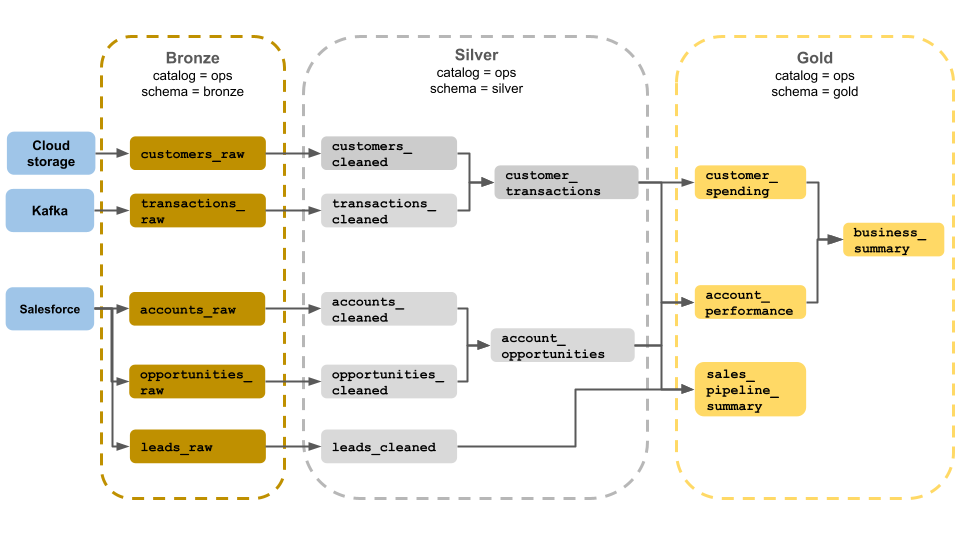
\includegraphics[width=0.78\textwidth]{figuras/medalhao-microsoft.png}
    \\[4pt]
    {\footnotesize Fonte: \citeonline{MicrosoftMedallion2024}.}
\end{figure}

\subsection{Formato Apache Parquet}
\label{subsec:parquet}

O Apache Parquet é um formato de armazenamento colunar mantido pela Apache Software Foundation \cite{ApacheParquet2024}. Nos formatos orientados a linha, como CSV ou JSON, todos os campos de um mesmo registro ficam juntos no disco; o Parquet inverte essa lógica e grava em sequência os valores de cada coluna. Uma consulta que usa poucas colunas lê apenas os blocos delas (\textit{column pruning}), e o ganho cresce com tabelas de dezenas de colunas e milhões de registros, como as deste trabalho. A \autoref{fig:parquet-layout} mostra a organização do arquivo definida pela especificação: as linhas são divididas em grupos (\textit{row groups}); dentro de cada grupo, cada coluna ocupa um bloco contíguo (\textit{column chunk}), dividido em páginas; e o rodapé (\textit{footer}) guarda o esquema e, para cada bloco, a posição no arquivo e estatísticas como mínimo e máximo.

\begin{figure}[htbp]
    \centering
    \caption{Organização de um arquivo Parquet}
    \label{fig:parquet-layout}
    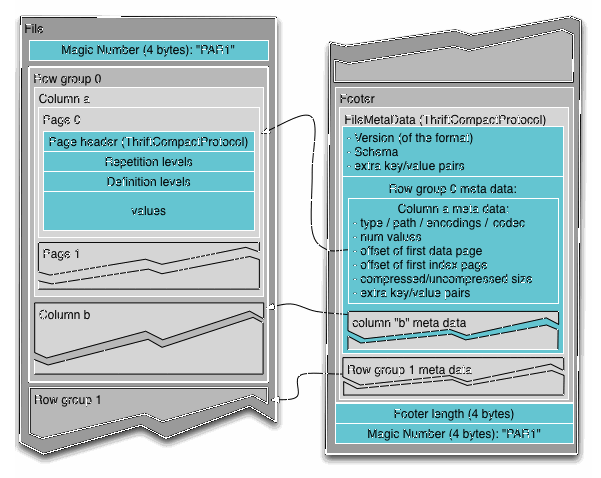
\includegraphics[width=0.55\textwidth]{figuras/parquet-layout-apache.png}
    \\[4pt]
    {\footnotesize Fonte: \citeonline{ParquetFormat2026}.}
\end{figure}

A leitura seletiva vem acompanhada de dois outros benefícios. No \textit{predicate pushdown}, os filtros são avaliados contra as estatísticas de mínimo e máximo guardadas nos metadados de cada bloco, e blocos inteiros são descartados sem leitura; pelos mesmos metadados, contar as linhas de um arquivo não exige ler nenhum dado. E a compressão é mais eficiente: valores de uma mesma coluna têm distribuição parecida, o que favorece algoritmos como Snappy e ZSTD, e o arquivo comprimido é consultado sem importação prévia. O formato aceita ainda particionar os arquivos por colunas como ano e estado, o que permite ao leitor carregar só as partições que casam com os filtros da consulta \cite{ApacheParquet2024}.

\subsection{DuckDB e repositórios públicos de dados}
\label{subsec:motores-in-process}

Os motores de \textit{Online Analytical Processing} (OLAP) tradicionais, como Redshift, BigQuery ou ClickHouse, seguem o modelo cliente-servidor, que cobra seu preço em latência de rede e complexidade de operação. Os motores \textit{in-process} são executados dentro do próprio processo da aplicação, sem servidor separado, e o DuckDB é o principal representante dessa categoria. Ele usa execução vetorizada: em vez de processar uma linha por vez, opera sobre vetores de valores de uma mesma coluna, o que aproveita as instruções vetoriais dos processadores modernos \cite{Raasveldt2019}.

\label{subsec:repositorios-dados}

Em vez de um \textit{bucket} de armazenamento de objetos, como o S3, este trabalho usa um repositório de dados versionado, o Hugging Face Hub \cite{HuggingFaceDatasets2026}. Cada conjunto de dados é um repositório com histórico de \textit{commits}: um envio cria uma nova versão, e as anteriores continuam recuperáveis. Os arquivos são servidos por HTTP com suporte a requisições parciais, o que permite ao DuckDB lê-los no próprio repositório pelo protocolo \texttt{hf://}, inclusive com padrões de \textit{glob} sobre as partições, sem cópia local \cite{DuckDB2024}.

A diferença em relação a um \textit{bucket} privado não é de desempenho, mas de papel. No \textit{bucket} privado, o \textit{data lake} é infraestrutura de trabalho, e publicar significa produzir uma segunda cópia; no repositório público, armazenamento e publicação são o mesmo lugar, sem uma cópia de trabalho e outra publicada que possam divergir. É o que os princípios FAIR pedem de dados de pesquisa: que sejam localizáveis, acessíveis, interoperáveis e reutilizáveis \cite{WilkinsonFair2016}.

Uma propriedade desse modelo tem consequência direta na engenharia: o envio é aditivo. Um \textit{commit} acrescenta ou substitui os arquivos enviados, mas não remove os que deixaram de existir na origem, a menos que a remoção seja pedida explicitamente \cite{HuggingFaceUpload2026}. Se uma camada for reorganizada e seus arquivos renomeados, as versões antigas permanecem, e uma leitura da pasta inteira passa a contá-las junto com as novas.

\subsection{Orquestração de \textit{pipelines}}
\label{subsec:orquestracao}

Um \textit{pipeline} de dados com várias etapas precisa de um orquestrador, que decide quando cada etapa roda e garante que ela só comece depois daquelas de que depende. Essa estrutura é um grafo acíclico dirigido (DAG), em que os nós são as etapas e as arestas, as dependências entre elas \cite{Reis2022}. Ferramentas dedicadas, como o Apache Airflow, implementam esse modelo, mas pressupõem um servidor próprio em funcionamento contínuo.

Plataformas de integração contínua oferecem os mesmos elementos como serviço. No GitHub Actions \cite{GitHubActions2026}, um \textit{workflow} é um arquivo de configuração versionado junto do código-fonte, composto de \textit{jobs} executados em máquinas virtuais efêmeras, os executores (\textit{runners}), criadas para a execução e descartadas ao final. Um \textit{workflow} pode ser disparado por agendamento, por alteração no código ou manualmente, e pode chamar outros como sub-rotinas reutilizáveis. A dependência declarada entre \textit{jobs} define o DAG, e a plataforma executa em paralelo os que não dependem uns dos outros. Para repositórios públicos, a execução não tem custo.

Duas características desse modelo condicionam o desenho do \textit{pipeline}. Os executores são isolados: um \textit{job} não enxerga o disco de outro, e todo dado que passa de uma etapa à seguinte precisa ser persistido fora do executor \cite{GitHubActions2026}. E cada execução tem memória, disco e duração limitados, o que favorece dividir o trabalho em unidades pequenas e independentes, que cabem no executor e podem ser repetidas isoladamente quando uma delas falha.

\subsection{Visualização \textit{web} sem servidor}
\label{sec:visualizacao}

Um \textit{dashboard} interativo na \textit{web} pode executar as consultas em um servidor ou no navegador de quem o visita. No primeiro caso, cada interação exige uma ida e volta pela rede, e a aplicação só existe enquanto houver um processo de servidor ativo; no segundo, o filtro responde sem rede, e o \textit{dashboard} se reduz a um conjunto de arquivos estáticos \cite{Kohn2022}.

A segunda arquitetura combina três peças. A interface é uma aplicação de página única, construída com uma biblioteca de componentes como o React \cite{React2026}, em que cada parte da tela é função declarada do estado: muda o filtro, e a biblioteca redesenha só o que depende dele. O motor é o DuckDB-Wasm \cite{Kohn2022}, o mesmo DuckDB compilado para WebAssembly, que executa SQL analítico sobre arquivos Parquet dentro do navegador. E, sem servidor de aplicação, o site pode ser hospedado em uma rede de distribuição de conteúdo, como o Cloudflare Pages \cite{CloudflarePages2026}, sem custo de processamento por visita. Os gráficos são declarados como configuração, e não desenhados passo a passo, em bibliotecas como o Apache ECharts \cite{Li2018}.

O desenho da interação segue o princípio formulado por \citeonline{Shneiderman1996} para sistemas de busca visual de informação: primeiro a visão geral, depois aproximação e filtro, e os detalhes sob demanda. Em um \textit{dashboard} analítico, isso se traduz em abrir cada tela pela resposta agregada, permitir recortar o dado (por período, território ou grupo) e deixar os valores exatos a um clique de cada gráfico.

\section{Séries temporais, previsão e \textit{nowcasting}}

Uma série temporal é uma sequência de observações de uma variável coletadas em intervalos regulares \cite{Hyndman2021}, que se costuma decompor em tendência, sazonalidade, ciclo e ruído \cite{Box2015}.

\label{subsec:sarima}

A família \textit{AutoRegressive Integrated Moving Average} (ARIMA), formalizada por \citeonline{Box2015}, modela uma série a partir de três mecanismos: a dependência da observação atual em relação às anteriores (componente autorregressiva, $p$), a diferenciação necessária para estabilizar o nível da série (componente integrada, $d$) e a dependência em relação aos erros passados (componente de média móvel, $q$). A extensão sazonal, SARIMA, replica esses mecanismos no período da sazonalidade e é escrita como
\begin{equation}
    \text{SARIMA}(p, d, q)(P, D, Q)_m,
\end{equation}
em que $(P, D, Q)$ são as ordens sazonais e $m$ é o período, igual a 12 nas séries mensais com ciclo anual.

A diferenciação sazonal ($D = 1$) é o que torna a família adequada à série de saldo de empregos: ela remove o ciclo anual de admissões e desligamentos subtraindo de cada mês o mesmo mês do ano anterior, em lugar de estimar uma forma funcional para esse ciclo \cite{Hyndman2021}. O preço é a perda dos primeiros $m$ pontos da série, o que importa quando o histórico é curto.

Uma alternativa de outra natureza é o Prophet \cite{Taylor2018}, que trata a série como uma regressão: uma tendência linear por partes, uma sazonalidade descrita por séries de Fourier e, quando houver, efeitos de feriados. Foi desenhado para séries de negócio com lacunas e mudanças de tendência, com poucos parâmetros a calibrar; o principal é a flexibilidade da tendência (\textit{changepoint prior scale}), que controla quanto a inclinação pode mudar. Em vez de diferenciar a série para remover o ciclo anual, como o SARIMA, o Prophet o estima diretamente.

\label{subsec:origem-movel}

Avaliar um modelo de série temporal por amostragem aleatória é inválido: embaralhar as observações permite ao modelo treinar com o futuro e prever o passado. A alternativa consagrada é a validação de origem móvel \cite{Tashman2000}, também chamada de validação em janelas expansivas: o modelo é treinado com os dados até um instante $T$, prevê os $h$ períodos seguintes, a origem avança e o procedimento se repete. O erro reportado é a média das dobras.

O \textit{baseline} de comparação precisa ser avaliado nas mesmas dobras e no mesmo horizonte, e uma grade grande de especificações, avaliada em poucas dobras, encontra por acaso o modelo que se sai bem naquelas dobras: é sobreajuste deslocado da amostra de treino para a de validação \cite{Tashman2000, Hyndman2021}. Um \textit{baseline} usual em séries sazonais é o ingênuo sazonal, que prevê para cada mês o valor do mesmo mês do ano anterior \cite{Hyndman2021}; um modelo que não o supera não se justifica.

\label{subsec:metricas}

A qualidade das previsões é medida por duas métricas clássicas \cite{Hyndman2021}. O \textit{Mean Absolute Error} (MAE) calcula o erro médio em valores absolutos, na mesma unidade da série. O \textit{Root Mean Squared Error} (RMSE) penaliza os erros de forma quadrática e, por isso, é mais sensível a previsões muito distantes do valor observado:

\begin{equation}
    \text{MAE} = \frac{1}{n}\sum_{i=1}^{n}|y_i - \hat{y}_i|
    \qquad
    \text{RMSE} = \sqrt{\frac{1}{n}\sum_{i=1}^{n}(y_i - \hat{y}_i)^2}
\end{equation}

onde $y_i$ é o valor observado e $\hat{y}_i$ é o valor previsto pelo modelo para o período $i$.

\label{subsec:nowcasting}

Nem toda pergunta sobre uma série é uma pergunta sobre o futuro. Estatísticas oficiais são publicadas com defasagem, e o valor do período corrente, ou mesmo do já encerrado, costuma ser desconhecido quando a decisão precisa ser tomada. O \textit{nowcasting}, formalizado por \citeonline{Giannone2008} para o PIB, estima esse presente a partir de informações divulgadas antes e com mais frequência que a estatística de interesse. \citeonline{Banbura2013} o definem como a previsão do presente, do passado muito recente e do futuro muito próximo, e mostram que o ganho vem do fluxo de publicação: cada dado que sai antes da estatística oficial reduz a incerteza sobre ela. A RAIS e o CAGED têm exatamente essa relação: o estoque anual é publicado no ano seguinte, e o fluxo mensal, poucas semanas depois de cada mês.

\section{Métodos de decomposição salarial e de sobrevivência}

As perguntas sobre qualidade do emprego e equidade não se respondem com extrapolação de série. Esta seção apresenta os dois métodos empregados para elas.

\label{subsec:oaxaca}

Proposta de forma independente por \citeonline{Oaxaca1973} e \citeonline{Blinder1973}, a decomposição de Oaxaca-Blinder separa a diferença média de salários entre dois grupos em duas parcelas. Partindo de uma regressão do logaritmo do salário sobre características produtivas em cada grupo, a diferença das médias se escreve
\begin{equation}
    \bar{Y}_A - \bar{Y}_B =
    \underbrace{(\bar{X}_A - \bar{X}_B)'\beta^{*}}_{\text{explicada}} +
    \underbrace{\bar{X}_A'(\hat{\beta}_A - \beta^{*}) + \bar{X}_B'(\beta^{*} - \hat{\beta}_B)}_{\text{não explicada}},
\end{equation}
em que $\bar{X}$ são as médias das características, $\hat{\beta}$ os coeficientes estimados em cada grupo e $\beta^{*}$ o vetor de referência.

A parcela explicada é a diferença atribuível ao fato de os grupos terem características distintas: escolaridade, experiência, ocupação, porte da empresa. A não explicada é a que permanece entre pessoas com características equivalentes, isto é, uma diferença de \textit{retorno} às mesmas características. A escolha de $\beta^{*}$ não é neutra, porque usar os coeficientes de um dos grupos altera a magnitude das parcelas; \citeonline{Neumark1988} propõe os coeficientes da regressão conjunta dos dois grupos, convenção adotada neste trabalho e discutida por \citeonline{Jann2008}.

A parcela não explicada não é medida de discriminação. Ela contém tudo que afeta o salário e não está no modelo: experiência anterior não registrada, interrupções de carreira, negociação, preferências por jornada. É um limite superior para o que a discriminação poderia explicar, e não uma estimativa dela \cite{Jann2008}.

\label{subsec:sobrevivencia}

A permanência em um emprego é um fenômeno de duração, e a análise de sobrevivência se aplica a ele. O estimador de \citeonline{Kaplan1958} é a ferramenta usual quando se acompanha uma coorte ao longo do tempo, tratando como censurados os casos cujo desfecho não foi observado.

Esse estimador, porém, é incompatível com a estrutura da RAIS, que é um corte transversal: cada edição retrata os vínculos existentes em 31 de dezembro, e não uma coorte seguida no tempo. Nesse retrato, vínculos longos estão sobre-representados, porque quem permanece muitos anos aparece em muitas edições, e quem passou poucos meses pode não aparecer em nenhuma; aplicar Kaplan-Meier a ele produz durações infladas \cite{Preston2001}.

A alternativa adequada é a tábua de vida de período, instrumento clássico da demografia \cite{Preston2001}. Ela toma as taxas de saída observadas em cada faixa de duração \textit{em um mesmo ano} e com elas constrói uma sobrevivência sintética: a probabilidade de permanência de uma coorte hipotética que experimentasse, ao longo da vida, as taxas daquele ano. A tábua descreve, portanto, o risco vigente no período, e não a trajetória de quem entrou em um ano específico.

\section{Trabalhos relacionados}
\label{sec:relacionados}

Entre os muitos estudos sobre o mercado de trabalho com a RAIS e o CAGED, esta seção apresenta os mais próximos deste, por método ou por objeto, e o que os diferencia.

\begin{table}[htbp]
    \centering
    \caption{Comparação entre os trabalhos relacionados e a proposta deste TCC}
    \label{tab:comparativo-relacionados}
    \footnotesize
    \renewcommand{\arraystretch}{1.35}
    \begin{tabularx}{\textwidth}{%
        >{\raggedright\arraybackslash\hsize=1.20\hsize}X
        >{\raggedright\arraybackslash\hsize=1.00\hsize}X
        >{\raggedright\arraybackslash\hsize=0.90\hsize}X
        >{\raggedright\arraybackslash\hsize=1.10\hsize}X
        >{\raggedright\arraybackslash\hsize=1.00\hsize}X
        >{\raggedright\arraybackslash\hsize=0.80\hsize}X}
        \toprule
        \rowcolor{black!8}
        \textbf{Trabalho} & \textbf{Fontes} & \textbf{Período} & \textbf{Recorte} & \textbf{Modelagem preditiva} & \textbf{Reprodu\-tível} \\
        \midrule
        \citeonline{IPEA2023} & PNAD, CAGED, RAIS  & Até 2023 & Todo o mercado & Não & Não \\
        \citeonline{Fecomercio2024} & RAIS & 2012--2022 & 30 ocupações de TI & Não & Não \\
        \citeonline{Brasscom2024} & RAIS, CAGED e outras & Anual & Macrossetor TIC & Projeção de déficit & Não \\
        \citeonline{Azambuja2016} & RAIS & 2006--2013 & Serviços TIC (CNAE) & Não & Parcial \\
        \citeonline{Dobner2022} & RAIS & 2012--2018 & Rio Grande do Sul & Não & Parcial \\
        \rowcolor{blue!6}
        \textbf{Este TCC} & RAIS e CAGED & 2007--2026 & TI por CBO e CNAE & SARIMA e \textit{nowcast} & Sim \\
        \bottomrule
    \end{tabularx}
    \\[4pt]
    {\footnotesize Fonte: Elaborado pelo autor.}
\end{table}

O Instituto de Pesquisa Econômica Aplicada (IPEA) publica relatórios trimestrais de \textit{Conjuntura do Mercado de Trabalho no Brasil}, que cruzam a Pesquisa Nacional por Amostra de Domicílios Contínua (PNAD Contínua), o CAGED e a RAIS \cite{IPEA2023}. O foco é macroeconômico (população ocupada, taxa de desemprego e rendimento médio em recortes amplos), sem aprofundar um setor específico como o de TI.

A pesquisa da FECOMERCIOSP \cite{Fecomercio2024} é a que mais se aproxima deste trabalho, mas descreve séries anuais de 30 ocupações, sem modelagem preditiva nem integração com o CAGED, e, publicada como nota técnica, não traz o detalhamento que permitiria reproduzi-la. Os relatórios da BRASSCOM \cite{Brasscom2024, Brasscom2025} combinam RAIS, CAGED e outras fontes, mas não abrem a metodologia nem os dados intermediários.

Na literatura acadêmica, \citeonline{Azambuja2016} usaram a RAIS de 2006 a 2013 para comparar a demanda de trabalho das empresas de serviços de TIC com a do setor de serviços como um todo, e concluíram que o setor é heterogêneo: as condições de trabalho variam conforme o grau de inserção de cada segmento na competição por inovação. No tema da equidade, \citeonline{Dobner2022} aplicaram as decomposições de Oaxaca-Blinder e de Ñopo à RAIS do Rio Grande do Sul, de 2012 a 2018, e encontraram hiato de gênero favorável aos homens em todos os setores, com uma característica notável: se os atributos produtivos determinassem o salário, as mulheres ganhariam mais. Nenhum dos dois trata o setor de TI pelas duas lentes, de setor e de ocupação, nem cobre a série desde 2007.

No campo técnico, a Arquitetura Medalhão (\autoref{subsec:medalhao}) tornou-se referência para a organização de \textit{data lakes}, e \citeonline{Armbrust2021} propuseram o \textit{lakehouse}, que combina o desempenho analítico do \textit{data warehouse} com o armazenamento de dados brutos em formatos abertos como o Parquet, lidos diretamente por motores analíticos modernos, a mesma intuição que orienta as escolhas técnicas deste trabalho. No acesso a microdados brasileiros, a iniciativa mais próxima é a Base dos Dados \cite{Dahis2022}, que publica dezenas de bases públicas já tratadas, entre elas a RAIS, em um \textit{data lake} de esquema unificado consultável por SQL no BigQuery. Este trabalho acrescenta o recorte setorial com as duas lentes, a recontagem publicada contra o dado bruto, a auditoria da fonte e a leitura por HTTP, sem conta em provedor de nuvem.

Esses trabalhos, comparados na \autoref{tab:comparativo-relacionados}, deixam três lacunas que este TCC pretende preencher: a integração das duas bases em uma série única e harmonizada, cobrindo dezoito anos; a aplicação de modelos formais (previsão da série mensal com especificação escolhida por validação de origem móvel e estimação do estoque corrente por \textit{nowcast}), além da análise descritiva; e uma plataforma analítica reprodutível, em que o \textit{pipeline} e o \textit{dashboard} podem ser inspecionados, executados e estendidos por outros pesquisadores.
